%\usebackgroundtemplate{%             declare it
	%	\tikz[overlay,remember picture] \node[opacity=1, at=(current page.center)] {
		%		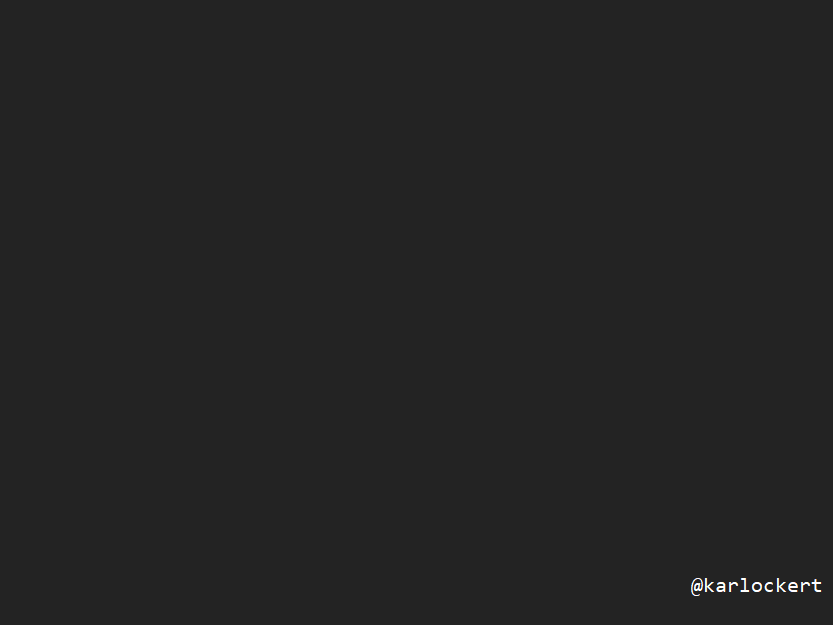
\includegraphics[height=\paperheight]{img/bakgrunn.png}};}

\begin{frame}[noframenumbering, plain]
	\begin{block}{\color{white}\textbf{\Large{
					%
					Topological Insulators - 1
					%	
		}}}
		\vspace{-10pt}\rule{\textwidth}{0.5pt}
		\color{white}
		
%		Topological insulators is a class of quantum matter with predicted properties relevant for the development of highly energy efficient information technologies such as spintronics.
		
		These materials are “topological” in the sense that certain quantities of the system is left invariant when it undergoes smooth transformations in the parameter space. An example of such a property is the Chern invariant $n$.
%		, which is associated with a quantized hall conductance. 
		
		This number can be calculated as the total Berry flux through the Brillouin zone from each band. 
		\begin{equation*}
			\label{eq:hamiltonian_pseudomagnetic}
			H(\bm{k}) = E_{\bm{k}}I + \vb d_{\bm{k}}\cdot\bm\sigma, 
		\end{equation*}
		the Chern number can be expressed in terms of the normalized vector $\hat{\vb{d}}_{\bm{k}} = \vb{d}_{\bm{k}} / |\vb{d}_{\bm{k}}|$ alone;
	
		
	\end{block}
	{\large
			\begin{equation*}
			n = \frac{1}{4\pi}\int_{1\text{BZ}}\dd[2]{\bm{k}}\hat{\vb{d}}_{\bm{k}} \cdot(\partial_{k_x}\hat{\vb{d}}_{\bm{k}}\cross\partial_{k_y}\hat{\vb{d}}_{\bm{k}}).
		\end{equation*}
	
	}
	
%	\begin{block}{}
%		\color{white}
%		
%		Some more information here
%		
%	\end{block}
\end{frame}


%\usebackgroundtemplate{%             declare it
	%	\tikz[overlay,remember picture] \node[opacity=1, at=(current page.center)] {
		%		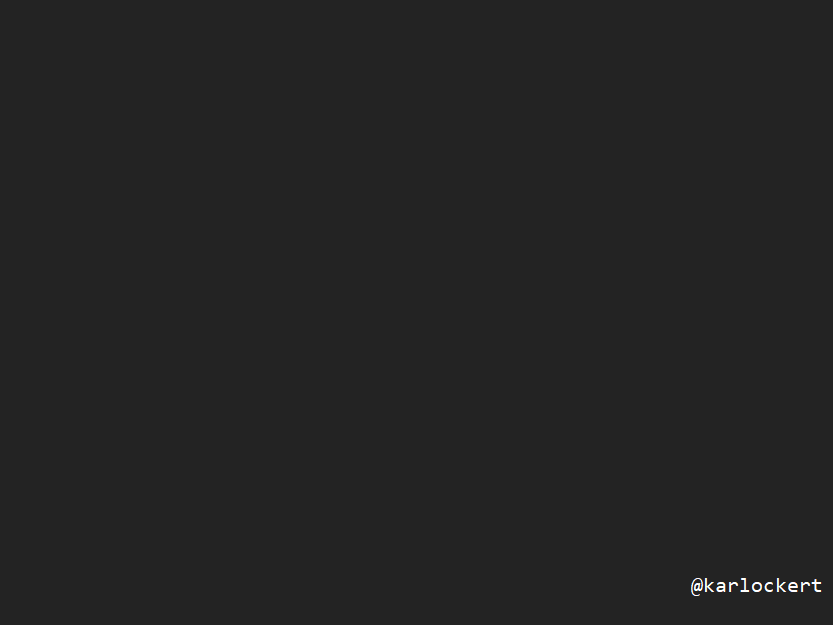
\includegraphics[height=\paperheight]{img/bakgrunn.png}};}

\begin{frame}[noframenumbering, plain]
	\begin{block}{\color{white}\textbf{\Large{
					%
					Topological Insulators - 2
					%	
		}}}
		\vspace{-10pt}\rule{\textwidth}{0.5pt}
		\color{white}
		
		%		Topological insulators is a class of quantum matter with predicted properties relevant for the development of highly energy efficient information technologies such as spintronics.
		
	
		Haldane showed in 1988 that for a particular model of the hexagonal lattice -- such as Graphene, the hall conductance is quantized in terms of this integer
	
		
	\end{block}
	{\large
		\begin{equation*}
		\sigma^{xy} = n\frac{2\pi e^2}{\hbar}
	\end{equation*}
		
	}
	
		\begin{block}{}
				\color{white}
				
				where the Chern number $n=0,\pm1$ is related to the number of edge states through what is now called the bulk-boundary correspondence. This model of spinless fermions on a hexagonal lattice is famously called the ``Haldane model''. The generalisation with spin degrees of freedom included led to the prediction of Spin Hall insulators -- a two dimensional rendition of a topological insulator.  
				
			\end{block}
\end{frame}
